\documentclass[journal]{IEEEtran}
\usepackage[a5paper, margin=10mm]{geometry}
%\usepackage{lmodern} % Ensure lmodern is loaded for pdflatex
\usepackage{tfrupee} % Include tfrupee package

%iffalse
\let\negmedspace\undefined
\let\negthickspace\undefined
\usepackage{gvv-book}
\usepackage{gvv}
\usepackage{cite}
\usepackage{amsmath,amssymb,amsfonts,amsthm}
\usepackage{algorithmic}
\usepackage{graphicx}
\usepackage{textcomp}
\usepackage{xcolor}
\usepackage{txfonts}
\usepackage{listings}
\usepackage{enumitem}
\usepackage{mathtools}
\usepackage{gensymb}
\usepackage{comment}
\usepackage[breaklinks=true]{hyperref}
\usepackage{tkz-euclide} 
\usepackage{listings}                                        
%\def\inputGnumericTable{}                                 
\usepackage[latin1]{inputenc}                                
\usepackage{color}                                            
\usepackage{array}                                            
\usepackage{longtable}                                       
\usepackage{calc}                                             
\usepackage{multirow}                                         
\usepackage{hhline}                                           
\usepackage{ifthen}                                           
\usepackage{lscape}
\usepackage{tabularx}
\usepackage{array}
\usepackage{float}
\usepackage{multicol}

\newcommand{\BEQA}{\begin{eqnarray}}
\newcommand{\EEQA}{\end{eqnarray}}
%\newcommand{\define}{\stackrel{\triangle}{=}}

\setlength{\headheight}{1cm} % Set the height of the header box
\setlength{\headsep}{0mm}     % Set the distance between the header box and the top of the text


%\usepackage[a5paper, top=10mm, bottom=10mm, left=10mm, right=10mm]{geometry}


\setlength{\intextsep}{10pt} % Space between text and floats

% Marks the beginning of the document
\begin{document}
\onecolumn
\bibliographystyle{IEEEtran}
\vspace{3cm}

%\renewcommand{\theequation}{\theenumi}
\numberwithin{equation}{enumi}
\numberwithin{figure}{enumi}
\renewcommand{\thefigure}{\theenumi}
\renewcommand{\thetable}{\theenumi}

\title{3-3.3-2}
\author{ai24btech11030 - Shiven Bajpai}
\maketitle

\renewcommand{\thefigure}{\theenumi}
\renewcommand{\thetable}{\theenumi}

\textbf{Question: } Construct a triangle with sides $5cm$, $6cm$ and $7cm$
\\

\textbf{Solution: } Let the vertices of triangle be $\vec{A}$, $\vec{B}$ and $\vec{C}$ and lengths of the sides opposing them be denoted by $a = 5cm$, $b = 6cm$ and $c = 7cm$ respectively.
\\

By Cosine rule in $\Delta ABC$,
\begin{align*}
	a^2 &= b^2 + c^2 - 2bc \cos A\\
	\cos A &= \frac{b^2 + c^2 - a^2}{2bc}\\
	\cos A &= \frac{60}{84}\\
\end{align*}

Let $\vec{A} = \vec{0}$ and $\vec{C} = \myvec{b \\ 0}$. Then $\vec{B} = c\myvec{\cos A \\ \sin A}$

Substituting values we get, $\vec{A} = \vec{0}, \vec{B} = \myvec{5 \\ \sqrt{24}}, \vec{C} = \myvec{6 \\ 0}$

\begin{figure}[H]
	\centering
	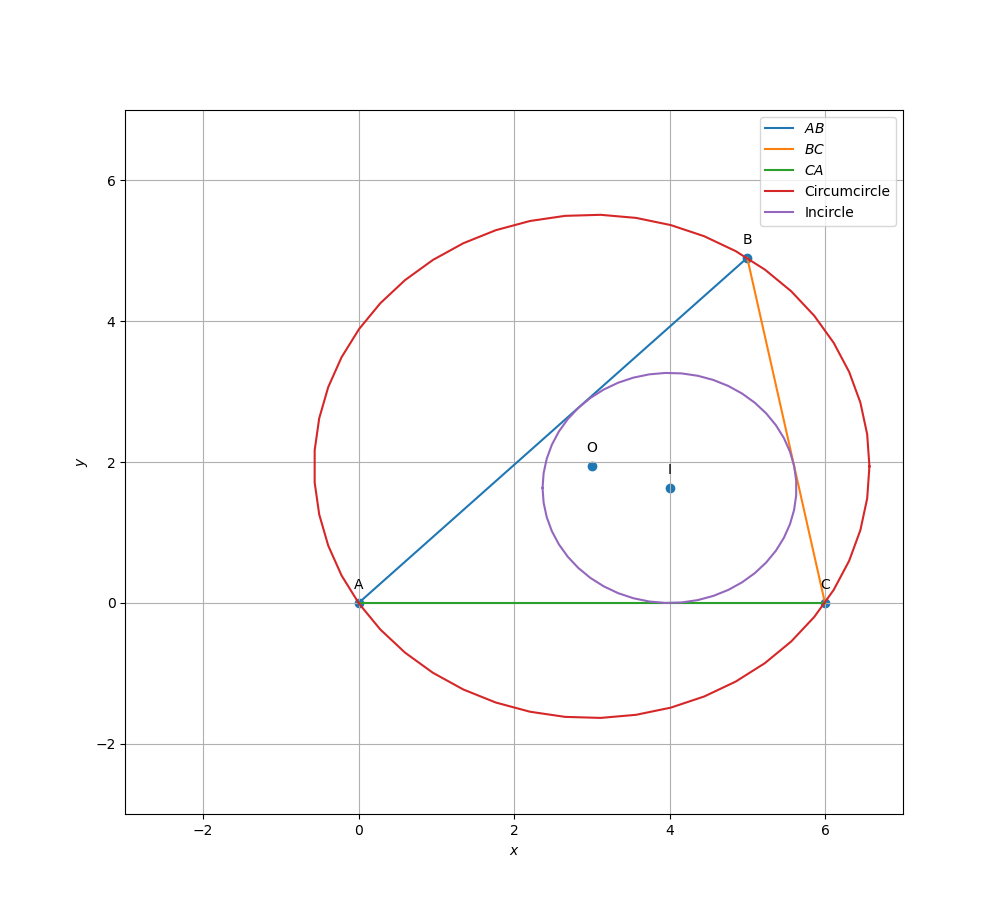
\includegraphics[width=0.75\columnwidth]{Figures/Figure.png}
	\label{fig}
\end{figure}

Code for this plot can be found at:
\begin{lstlisting}
    Codes/main.py
    Codes/main.c
\end{lstlisting}

\end{document}
